\documentclass[runningheads]{llncs}

\usepackage[T1]{fontenc}
\usepackage{graphicx}

% to display URLs in blue roman font according to Springer's eBook style:
%\usepackage{color}
%\renewcommand\UrlFont{\color{blue}\rmfamily}
%\urlstyle{rm}

\begin{document}
\title{Computer Networks Project \\ Romanian railways}

\author{P. Braha\inst{1}\orcidID{0009-0001-3636-2455}}
\authorrunning{F. Author et al.}
\institute{Alexandru Ioan Cuza University, Iasi IS 700221, Romania
\email{petrubraha@gmail.com}\\
\url{https://github.com/petru-braha}}

\maketitle
%
\begin{abstract} This work contains an overview of client-server paradigm, and a custom implementation of the application level 
The abstract should briefly summarize the contents of the paper in
150--250 words.

\keywords{First keyword  \and Second keyword \and Another keyword.}
\end{abstract}

%%------------------------------------------------
%%------------------------------------------------

\section{Introduction}

There will be presented the application level's API and some optimizations for speed

requirements
application level



transport level
speed 
corectness 
security

\subsection{Motivation}

Laboratory work. 

\subsubsection{Sample Heading (Third Level)} Only two levels of
headings should be numbered. Lower level headings remain unnumbered;
they are formatted as run-in headings.

\paragraph{Sample Heading (Fourth Level)}
The contribution should contain no more than four levels of
headings. Table~\ref{tab1} gives a summary of all heading levels.

\begin{table}
\caption{Table captions should be placed above the
tables.}\label{tab1}
\begin{tabular}{|l|l|l|}
\hline
Heading level &  Example & Font size and style\\
\hline
Title (centered) &  {\Large\bfseries Lecture Notes} & 14 point, bold\\
1st-level heading &  {\large\bfseries 1 Introduction} & 12 point, bold\\
2nd-level heading & {\bfseries 2.1 Printing Area} & 10 point, bold\\
3rd-level heading & {\bfseries Run-in Heading in Bold.} Text follows & 10 point, bold\\
4th-level heading & {\itshape Lowest Level Heading.} Text follows & 10 point, italic\\
\hline
\end{tabular}
\end{table}


\noindent Displayed equations are centered and set on a separate
line.
\begin{equation}
x + y = z
\end{equation}
Please try to avoid rasterized images for line-art diagrams and
schemas. Whenever possible, use vector graphics instead (see
Fig.~\ref{fig1}).

\begin{figure}
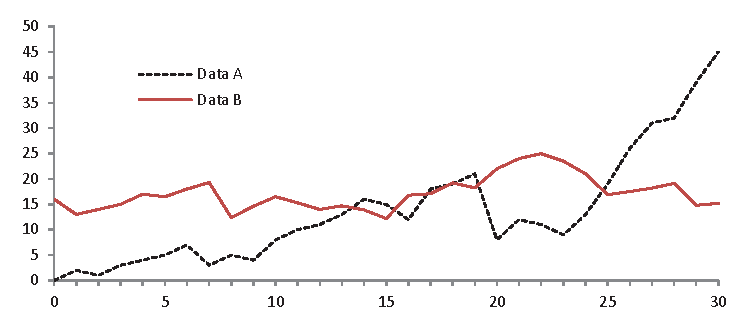
\includegraphics[width=\textwidth]{fig1.eps}
\caption{A figure caption is always placed below the illustration.
Please note that short captions are centered, while long ones are
justified by the macro package automatically.} \label{fig1}
\end{figure}

\begin{theorem}
This is a sample theorem. The run-in heading is set in bold, while
the following text appears in italics. Definitions, lemmas,
propositions, and corollaries are styled the same way.
\end{theorem}
%
% the environments 'definition', 'lemma', 'proposition', 'corollary',
% 'remark', and 'example' are defined in the LLNCS documentclass as well.
%
\begin{proof}
Proofs, examples, and remarks have the initial word in italics,
while the following text appears in normal font.
\end{proof}
For citations of references, we prefer the use of square brackets
and consecutive numbers. Citations using labels or the author/year
convention are also acceptable. The following bibliography provides
a sample reference list with entries for journal
articles~\cite{ref_article1}, an LNCS chapter~\cite{ref_lncs1}, a
book~\cite{ref_book1}, proceedings without editors~\cite{ref_proc1},
and a homepage~\cite{ref_url1}. Multiple citations are grouped
\cite{ref_article1,ref_lncs1,ref_book1},
\cite{ref_article1,ref_book1,ref_proc1,ref_url1}.

\begin{credits}
\subsubsection{\ackname} A bold run-in heading in small font size at the end of the paper is
used for general acknowledgments, for example: This study was funded
by X (grant number Y).

\subsubsection{\discintname}
It is now necessary to declare any competing interests or to specifically
state that the authors have no competing interests. Please place the
statement with a bold run-in heading in small font size beneath the
(optional) acknowledgments\footnote{If EquinOCS, our proceedings submission
system, is used, then the disclaimer can be provided directly in the system.},
for example: The authors have no competing interests to declare that are
relevant to the content of this article. Or: Author A has received research
grants from Company W. Author B has received a speaker honorarium from
Company X and owns stock in Company Y. Author C is a member of committee Z.
\end{credits}

\section{Applied Technologies}

Applied Technologies: Detail the specific technologies used (for example, TCP, UDP, etc.), with an emphasis on aspects relevant to the project. Explain the motivations behind the selection of these technologies.


\section{Application Structure}

diagram
3. Application Structure: Expose the concepts used in modeling and present a detailed diagram of the application.
Create an application that provides or updates real time information from all registered customers for: train schedule, departure status, delays and estimated arrival. The server reads the data from XML files and updates the data (delays and estimated arrivals) on clients request. All the logic will be realized in the server, the client just asks for information about departures/arrivals and sends information to the server about possible delays and estimated arrivals.


- sending from the server the information about the trains running on the day
- sending from the server information about departures in the next hour (according to plan, late by x min) only on request of a client
- sending from the server information about arrivals in the next hour (according to plan, x min late, x min early) only on request of a client

\section{Implementation Aspects}

describe the api
Implementation Aspects: Present specific and innovative sections of the project code, providing adequate documentation; present the application-level protocol you will implement; describe real usage scenarios.

\section{Conclusions}

tcp and udp protocol


\subsection{speed}

tcp/udp
i/o multiplexing
concurrency

\subsection{corectness}

tcp protocol

\subsection{security}

%%------------------------------------------------
%%------------------------------------------------

% \bibliographystyle{splncs04}
% \bibliography{mybibliography}

\begin{thebibliography}{8}
\bibitem{ref_article1}
Author, F.: Article title. Journal \textbf{2}(5), 99--110 (2016)

\bibitem{ref_lncs1}
Author, F., Author, S.: Title of a proceedings paper. In: Editor,
F., Editor, S. (eds.) CONFERENCE 2016, LNCS, vol. 9999, pp. 1--13.
Springer, Heidelberg (2016). \doi{10.10007/1234567890}

\bibitem{ref_book1}
Author, F., Author, S., Author, T.: Book title. 2nd edn. Publisher,
Location (1999)

\bibitem{ref_proc1}
Author, A.-B.: Contribution title. In: 9th International Proceedings
on Proceedings, pp. 1--2. Publisher, Location (2010)

\bibitem{ref_url1}
LNCS Homepage, \url{http://www.springer.com/lncs}, last accessed 2023/10/25
\end{thebibliography}
\end{document}
